\begin{table}[t]
\centering
\footnotesize
\begin{tabular}{|l|l|}
\hline
  \textbf{Platform} & \textbf{Nvidia GTX 780TI} \footnotemark{} \\ \hline
  \begin{tabular}[c]{@{}l@{}}Warp size\\ \# of SM cores\\ Execution model\\
                              Max warps per SM\\ Size of register file\\ \# of register banks\\
                              Warp scheduler\end{tabular}
                              & \begin{tabular}[c]{@{}l@{}}32\\ 16\\ In-order\\
                              64\\ 256KB (per SM)\\ 24\\
                              Greedy then oldest\end{tabular} \\ \hline
  \begin{tabular}[c]{@{}l@{}}Shared memory\\ L1 Cache\end{tabular}
                              & \begin{tabular}[c]{@{}l@{}}48KB\\ 16KB\end{tabular} \\ \hline
  L2 Cache & 1536KB \\ \hline
\end{tabular}
\caption{Platform parameters}
\label{tab:metho:platform}
\end{table}
\footnotetext{GPU architecture parameter from \mycite{APCM}}

\section{Methodology}
We evaluate the proposed scheme using GPGPU-Sim~\mycite{bakhoda2009analyzing}. 
Table~\ref{tab:metho:DRAMparam} shows the configuration we used for the simulation. We assume HBM2 device architecture based on a recent HBM2 design~\mycite{HynixHBM2, IMW17} with pseudo-channel mode enabled. 
We evaluated proposed DRAM architecture based on GTX780-TI device replacing timing model of HBM2 device
with existing timing model on DRAM system configuration of the GPGPU-sim, which originally modeled on GDDR5.  
This GPGPU-sim model coupled with HBM2 is a 1/4 scale down version of the Nvidia P100~\mycite{P100}, a product using HBM2 devices.

\def\arraystretch{1.2}
\begin{table}[!t]
\centering
\footnotesize
\begin{tabular}{|l|l|}
  \hline
  \multicolumn{2}{|c|}{\textbf{DRAM System parameters}} \\ \hline
    Channel/Device  & 8 \\ \hline
    Slices/Device   & 4-Hi \\ \hline
    Banks/Channel   & 32 \\ \hline
    Clock frequency & 1000MHz \\ \hline
    Burst length    & 4 \\ \hline
    DQ              & $\times128$  \\ \hline
\end{tabular}
\caption{DRAM system parameters}
\label{tab:metho:DRAMparam}
\end{table}

\def\arraystretch{1.2}
\begin{table}[!t]
\footnotesize
\centering
\begin{tabular}{|c|c|}
  \hline
	\multirow{3}{*}{\textbf{HBM2}} & {\textbf{1024b @ 1000MHz (ns)}}  \\ \cline{2-2}
		& {$t_{RP}$ = 16, $t_{RC}$ = 45, $t_{RAS}$ = 29, $t_{RCD}/2$ = 8,} \\
		& {$t_{CCDS} = 2$, $t_{CCDL} = 10$, $t_{RRD}$ = 2, $t_{WR}$ = 15, $t_{CL}$ = 12} \\ \hline
\end{tabular}
\caption{HBM2 timing parameters}
\label{tab:metho:HBM2param}
\end{table}

We evaluate the performance impact of our scheme across several GPU workloads 
including memory-intensive general-purpose workloads.
We run both popular deep learning workloads on Caffe~\mycite{caffe} 
(augmented with the in-house cuDNN-like library) 
and several GPU workloads including various memory-intensive workloads from Rodinia~\mycite{rodinia}.
To evaluate energy efficiency, we utilize the GPUWattch~\mycite{GPUWattch} integrated with GPGPU-Sim. 
For DRAM energy parameters, we take numbers from~\mycite{subchannel17}. 
Lastly, we estimate the area overhead of the proposed scheme using CACTI-3DD~\mycite{cacti3dd}.

\newpage
\section{DRAM Energy Savings}
Figure~\ref{fig:ch4:act_e_cnn} and \ref{fig:ch4:act_e_cnn} compare the DRAM activation energy of the baseline full activation, Half-DRAM~\mycite{Zhang14}, and our work with 4 and 8 \textit{sectors}. To first order, the activation energy is proportional to the number of columns activated. The activation energy savings are 37\%, 59\% and 76\% on average for Half-DRAM, and our work with 4 and 8 {\it sectors}, respectively, over the baseline. The energy savings are particularly pronounced for the workloads with frequent row buffer conflicts. In other word, lower spatial locality on a row buffer leads to greater savings of the activation energy. The CNN and MLP workloads have relatively lower row buffer locality to save activation energy about 75\% on average for the {\it 8-sector} configuration. Among Rodinia benchmarks streamcluster and hotspot have smaller savings due to the higher average row buffer locality.

\begin{figure}[t]
\centering
	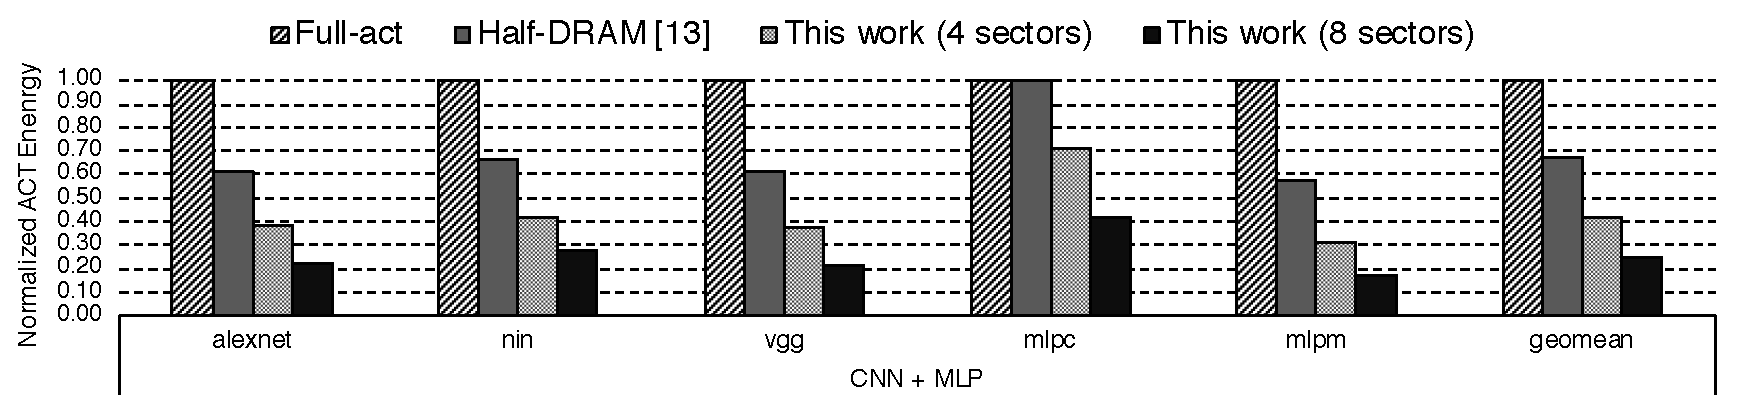
\includegraphics[width=\linewidth, page=1]{figure/thesis-eval.pdf}
\caption{Activation energy savings on CNN and MLP workloads}
\label{fig:ch4:act_e_cnn}
\end{figure}

\begin{figure}[t]
    \centering
		\includegraphics[width=\linewidth, page=2]{figure/thesis-eval.pdf}
    \caption{Activation energy savings on general workloads (Rodinia and STREAM)}
    \label{fig:ch4:act_e_gen}
\end{figure}

Occasionally, the activation energy savings are affected by row buffer access patterns. For instance, memory accesses in mlpc frequently fall on both halves of a row buffer. This leads to little activation energy savings with the Half-DRAM configuration. Figure~\ref{fig:ch4:DRAM_e_cnn} and \ref{fig:ch4:DRAM_e_gen} show how the activation energy savings are translated to DRAM-wide energy savings. The {\it 8-sector} configuration achieves 7.6\% energy savings on average with maximum savings of 14.1\%.

\begin{figure}[t]
    \centering
        \includegraphics[width=\linewidth, page=3]{figure/thesis-eval.pdf}
    \caption{DRAM energy savings on CNN and MLP workloads}
    \label{fig:ch4:DRAM_e_cnn}
\end{figure}

\begin{figure}[t]
    \centering
        \includegraphics[width=\linewidth, page=4]{figure/thesis-eval.pdf}
    \caption{DRAM energy savings on general workloads (Rodinia and STREAM)}
    \label{fig:ch4:DRAM_e_gen}
\end{figure}

\section{Performance Impact}
%Workload characteristics
Figure~\ref{fig:ch4:perf_cnn} demonstrates that both CNN and MLP workloads are tolerant of increased memory latency. The CNN workloads are known to compute-intensive as convolution layers, which dominates the execution time of a CNN, have a lot of data reuse~\mycite{jouppi2017tpu} to have relatively low off-chip memory access rate. Thus, they are able to maintain a high degree of memory-level parallelism and hence IPC. In contrast, MLP workloads, which are composed of fully-connected layers only, are known to be memory-intensive as there is no reuse of weight parameters in these layers. However, compared with recent results from Google's TPU~\mycite{jouppi2017tpu}, our MLP workloads are less memory-intensive due to fewer layers and smaller input data sets (Cifar-10 and MNIST). MLP workloads also have a lot of memory-level parallelism and is not sensitive to memory latency. Overall, both CNN and MLP workloads show only negligible IPC degradation.

\begin{figure}[t]
    \centering
        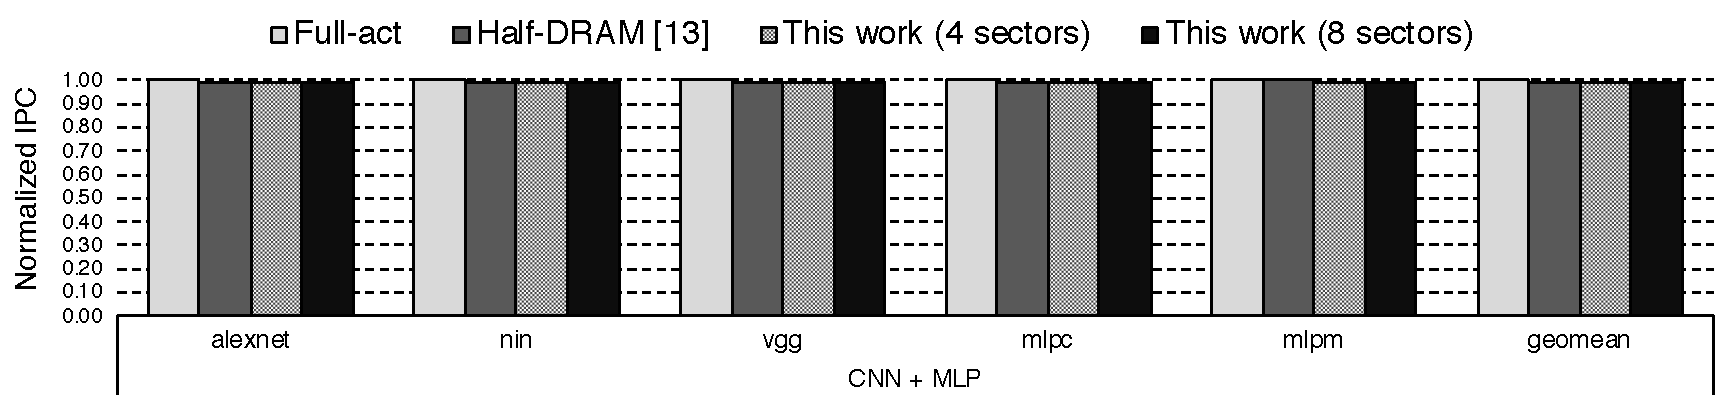
\includegraphics[width=\linewidth]{figure/perf-1.pdf}
    \caption{Performance degradation on CNN and MLP workloads}
    \label{fig:ch4:perf_cnn}
\end{figure}

\begin{figure}[t]
    \centering
        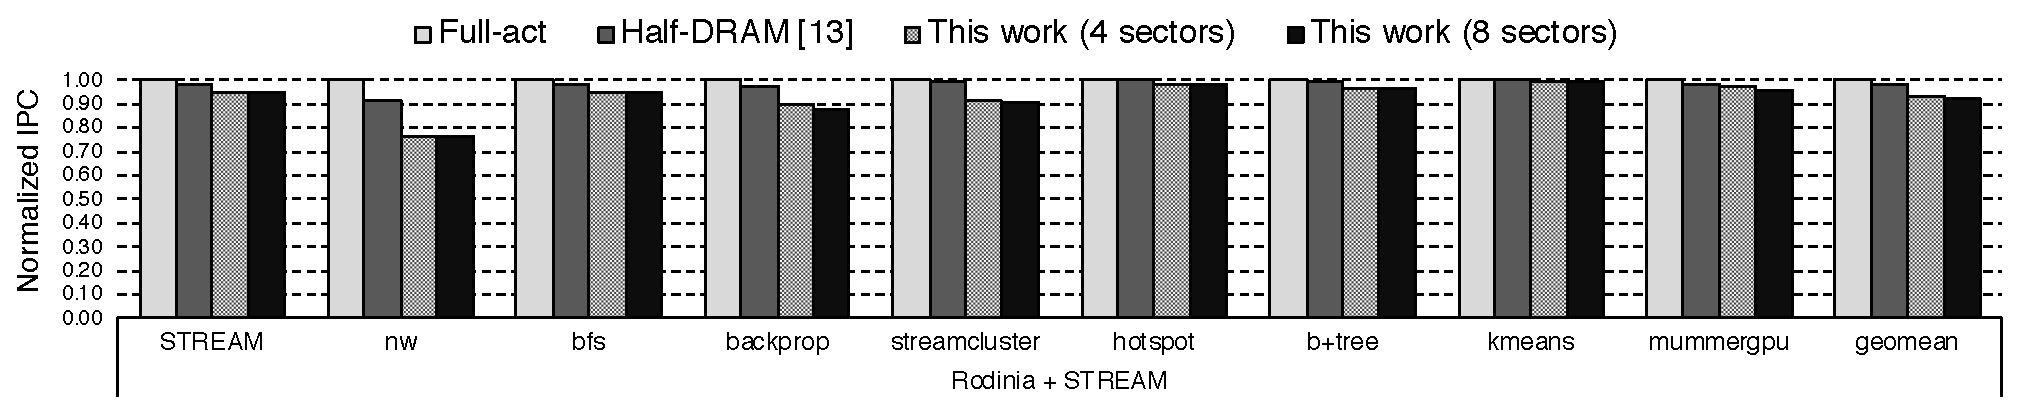
\includegraphics[width=\linewidth]{figure/perf-2.pdf}
    \caption{Performance degradation on general workloads (Rodinia and STREAM)}
    \label{fig:ch4:perf_gen}
\end{figure}

%Rodinia characteristics
To evaluate performance impact on non-DNN workloads we take memory-intensive GPU workloads from Rodinia~\mycite{rodinia} as shown on Figure~\ref{fig:ch4:perf_gen}. These workloads have a lower degree of memory-level parallelism than DNN workloads. For instance, needleman-wunsch (nw) has a fairly complex control flow with frequent branch divergence, thus suffering up to 22\% IPC degradation with the proposed scheme. In contrast, other workloads, such as hotspot, kmeans, and streamcluster, are compute-intensive with a high degree of memory-level parallelism, thus experiencing less performance hit than the others.


%Bank structure latency overhead
The IPC degradation is attributed to a couple of reasons. First, due to the narrower datapath between a DRAM mat and the I/O, the column access time (\texttt{tAA}) is increased substantially. This also negatively affects the latency of a column read/write request directed to the same bank as the previous column request. Second, there is an additional latency cost (8ns in our setup) when a new {\it sector} needs to be activated in the currently open row. Our proposed DRAM device activates the requested {\it sector} lazily only when a column request is directed to it. By activating only those {\it sectors} that are actually read or written, we may have a performance hit for workloads with good spatial locality in DRAM accesses. This problem may be alleviated by increasing the {\it sector} granularity (e.g., from 8 {\it sectors} to 4 {\it sectors} per DRAM row), while losing some of the energy savings with potential overfetching within a {\it sector}.

\section{Area Overhead}
We estimated area overhead incurred by additional circuitry using CACTI-3DD~\mycite{cacti3dd}.
The area overhead for the portion added to the inside of the dram core includes the following:
latches which hold valid bit vector per bank, and 9 AND gates added per subarray.
The \textit{sector} selection latch logic is modeled based on the local sense amplifier inside the core, 
and the NAND gate uses the NAND gate model used in the core.
Overall, the die area overhead is 0.3\% which we believe acceptable.
